% !TEX root = ../presentation.tex
% =============================================================
%  Chapter — Symbol Library
%  IEC 60617 / IEC 62747 symbols and single-line diagrams drawn with
%  Glyphwright: overview, transformers, switchgear and apparatus, VSC
%  converter with signal notation, rotation and mirroring, signal selection
%  in the LaTeX document, and two
%  single-line diagrams (transformer bay, converter station).
%  Symbols are drawn live with TikZ: figures/glyphwright-deck.tex holds the
%  Glyphwright \pic library, figures/*.tex the figure snippets; both are
%  generated from the Glyphwright repository (see figures/figures.yaml).
% =============================================================
\sectionslide{Symbol Library}{IEC symbols and single-line diagrams from one master geometry}

% Glyphwright symbol library (TikZ \pic definitions) and figure shorthand
%% glyphwright-deck.tex -- generated by Glyphwright tools/deck_figures.py, do not edit
%% \input this once in the document (TikZ must be loaded); then \pic {gw/<id>}
%% stroke classes (ISO 128, group 0.35)
\tikzset{
  gw/thin/.style={line width=0.25mm, line cap=round, line join=round},
  gw/normal/.style={line width=0.35mm, line cap=round, line join=round},
  gw/thick/.style={line width=0.7mm, line cap=round, line join=round},
  gw/solid/.style={draw=none},
  gw/small/.style={font=\fontsize{1.8mm}{2.2mm}\selectfont\sffamily, inner sep=0.3mm},
  gw/label/.style={font=\fontsize{2.5mm}{3mm}\selectfont\sffamily, inner sep=0.3mm},
  gw/title/.style={font=\fontsize{3.5mm}{4.2mm}\selectfont\sffamily, inner sep=0.3mm},
  gw/c-voltage/.style={color=gwvoltage},
  gw/c-current/.style={color=gwcurrent},
}
\definecolor{gwvoltage}{RGB}{31,95,191}
\definecolor{gwcurrent}{RGB}{200,30,30}
%% editable texts: \pic[gw/text={field=value, ...}] ... ; unset fields keep the default
\pgfkeys{/gw/text/.unknown/.code={\expandafter\def\csname gw@t@\pgfkeyscurrentname\endcsname{#1}}}
\tikzset{gw/text/.code={\pgfqkeys{/gw/text}{#1}}}
\newcommand\gwtext[2]{\ifcsname gw@t@#1\endcsname\csname gw@t@#1\endcsname\else#2\fi}
%% component data (label, e.g. vector group or "VSC"): \pic[gw/no label] hides it
\newif\ifgwlabel \gwlabeltrue
\tikzset{gw/no label/.code={\gwlabelfalse}}
\newcommand\gwlabel[1]{\ifgwlabel#1\fi}
%% signals (e.g. of the VSC converter), per pic or per diagram element:
%%   gw/signals={udpp, id_p}      show only these (all / none also work)
%%   gw/hide signals={id_n}       hide these
%%   gw/sig/udpp/.style={...}     style of one signal (colour, line style, ...)
%%   gw/element/U1/.style={...}   options for element U1 of a generated diagram
\newif\ifgwonly \gwonlyfalse
\newcount\gwsiggen   % each gw/signals starts a new list: the last one given wins
\pgfkeys{/gw/sel/.unknown/.code={\expandafter\def\csname gwsig@on@\the\gwsiggen @\pgfkeyscurrentname\endcsname{}},
         /gw/sel/all/.code={\gwonlyfalse},
         /gw/sel/none/.code={},
         /gw/unsel/.unknown/.code={\expandafter\def\csname gwsig@off@\pgfkeyscurrentname\endcsname{}}}
\tikzset{gw/signals/.code={\advance\gwsiggen by 1\relax\gwonlytrue\pgfqkeys{/gw/sel}{#1}},
         gw/hide signals/.code={\pgfqkeys{/gw/unsel}{#1}},
         gw/sigstyle/.code={\pgfkeysifdefined{/tikz/gw/sig/#1/.@cmd}{\pgfkeysalso{/tikz/gw/sig/#1}}{}},
         gw/element/.code={\pgfkeysifdefined{/tikz/gw/element/#1/.@cmd}{\pgfkeysalso{/tikz/gw/element/#1}}{}}}
\newcommand\gwsig[2]{\ifcsname gwsig@off@#1\endcsname\else
  \ifgwonly\ifcsname gwsig@on@\the\gwsiggen @#1\endcsname#2\fi\else#2\fi\fi}

\tikzset{gw/fig/.style={}}

%% glyphwright-symbols.tex -- generated, do not edit by hand

% Transformer, two windings, YNd11, HV neutral earthed, on-load tap changer
%   IEC 60617 06-09-02  transformer, two windings (form 2, circles)
%   IEC 60617 06-01-02  winding, star connection
%   IEC 60617 06-01-04  winding, delta connection
%   IEC 60617 02-03-01  variability / adjustability, general (tap changer arrow)
\tikzset{gw/xfmr2-YNd11-e1-oltc/.pic={
  \draw[gw/normal] (-3.750mm,0.000mm) circle [radius=5.000mm];
  \draw[gw/thin] (-3.750mm,0.000mm) -- (-3.750mm,2.000mm);
  \draw[gw/thin] (-3.750mm,0.000mm) -- (-5.482mm,-1.000mm);
  \draw[gw/thin] (-3.750mm,0.000mm) -- (-2.018mm,-1.000mm);
  \draw[gw/normal] (3.750mm,0.000mm) circle [radius=5.000mm];
  \draw[gw/thin] (3.750mm,2.000mm) -- (2.018mm,-1.000mm) -- (5.482mm,-1.000mm) -- cycle;
  \draw[gw/normal] (-8.750mm,0.000mm) -- (-12.500mm,0.000mm);
  \coordinate (-hv) at (-12.500mm,0.000mm);
  \draw[gw/normal] (8.750mm,0.000mm) -- (12.500mm,0.000mm);
  \coordinate (-lv) at (12.500mm,0.000mm);
  \draw[gw/normal] (-3.750mm,0.000mm) -- (-3.750mm,-5.000mm);
  \draw[gw/normal] (-3.750mm,-5.000mm) -- (-3.750mm,-7.500mm);
  \draw[gw/normal] (-6.250mm,-7.500mm) -- (-1.250mm,-7.500mm);
  \draw[gw/normal] (-5.250mm,-8.750mm) -- (-2.250mm,-8.750mm);
  \draw[gw/normal] (-4.250mm,-10.000mm) -- (-3.250mm,-10.000mm);
  \draw[gw/thin] (7.778mm,-7.778mm) -- (-7.778mm,7.778mm);
  \fill[gw/solid] (-7.778mm,7.778mm) -- (-6.859mm,5.869mm) -- (-5.869mm,6.859mm) -- cycle;
  \node[gw/label, anchor=south] at (0.000mm,7.500mm) {\gwlabel{YNd11}};
  \coordinate (-hv_centre) at (-3.750mm,0.000mm);
  \coordinate (-lv_centre) at (3.750mm,0.000mm);
  \coordinate (-label) at (0.000mm,7.500mm);
  \coordinate (-tag) at (0.000mm,-5.000mm);
}}

% Circuit breaker, open
%   IEC 60617 07-02-01  make contact (switch, general)
%   IEC 60617 07-13-05  circuit breaker
\tikzset{gw/cb/.pic={
  \draw[gw/normal] (0.000mm,5.000mm) -- (0.000mm,2.500mm);
  \coordinate (-a) at (0.000mm,5.000mm);
  \draw[gw/normal] (0.000mm,-5.000mm) -- (0.000mm,-2.500mm);
  \coordinate (-b) at (0.000mm,-5.000mm);
  \draw[gw/normal] (0.000mm,-2.500mm) -- (-2.500mm,1.830mm);
  \draw[gw/normal] (-0.750mm,1.750mm) -- (0.750mm,3.250mm);
  \draw[gw/normal] (-0.750mm,3.250mm) -- (0.750mm,1.750mm);
  \coordinate (-label) at (3.750mm,0.000mm);
  \coordinate (-tag) at (-3.750mm,0.000mm);
}}

% VSC HVDC converter, notation layout with signals
%   IEC 60617 02-15-01  earth, general
%   IEC 62747 clause 4  voltage-sourced converter (VSC) for HVDC (verify against Figure 2)
%   IEC 60617 06-14-03  converter (a.c./d.c.), general (verify)
\tikzset{gw/vsc2-sig/.pic={
  \draw[gw/normal] (-10.000mm,-16.250mm) -- (10.000mm,-16.250mm) -- (10.000mm,16.250mm) -- (-10.000mm,16.250mm) -- cycle;
  \draw[gw/thin] (-10.000mm,16.250mm) -- (10.000mm,0.000mm) -- (-10.000mm,-16.250mm);
  \draw[gw/thin] (-6.625mm,0.000mm) ++(0.00:1.125mm) arc [start angle=0.00, end angle=180.00, radius=1.125mm];
  \draw[gw/thin] (-4.375mm,0.000mm) ++(180.00:1.125mm) arc [start angle=180.00, end angle=360.00, radius=1.125mm];
  \draw[gw/thin] (2.750mm,10.125mm) -- (7.250mm,10.125mm);
  \draw[gw/thin] (2.750mm,8.625mm) -- (7.250mm,8.625mm);
  \draw[gw/thin] (2.750mm,-8.625mm) -- (7.250mm,-8.625mm);
  \draw[gw/thin] (2.750mm,-10.125mm) -- (7.250mm,-10.125mm);
  \draw[gw/normal] (-10.000mm,0.000mm) -- (-15.000mm,0.000mm);
  \coordinate (-ac) at (-15.000mm,0.000mm);
  \draw[gw/normal] (0.000mm,16.250mm) -- (0.000mm,20.000mm) -- (25.000mm,20.000mm);
  \coordinate (-dc1) at (25.000mm,20.000mm);
  \draw[gw/normal] (0.000mm,-16.250mm) -- (0.000mm,-20.000mm) -- (25.000mm,-20.000mm);
  \coordinate (-dc2) at (25.000mm,-20.000mm);
  \node[gw/label, anchor=east] at (-12.500mm,-8.125mm) {\gwlabel{\gwtext{label}{VSC}}};
  \gwsig{udpe_p}{\draw[gw/thin, gw/c-voltage, gw/sigstyle=udpe_p] (0.000mm,20.750mm) -- (0.000mm,25.000mm);}
  \gwsig{udpe_p}{\fill[gw/solid, gw/c-voltage, gw/sigstyle=udpe_p] (0.000mm,25.000mm) -- (-0.700mm,23.000mm) -- (0.700mm,23.000mm) -- cycle;}
  \gwsig{udpe_p}{\draw[gw/normal, gw/sigstyle=udpe_p] (2.500mm,26.250mm) -- (-2.500mm,26.250mm);}
  \gwsig{udpe_p}{\draw[gw/normal, gw/sigstyle=udpe_p] (1.500mm,27.500mm) -- (-1.500mm,27.500mm);}
  \gwsig{udpe_p}{\draw[gw/normal, gw/sigstyle=udpe_p] (0.500mm,28.750mm) -- (-0.500mm,28.750mm);}
  \gwsig{udpe_p}{\node[gw/label, gw/c-voltage, anchor=east, gw/sigstyle=udpe_p] at (-1.250mm,22.500mm) {\gwtext{udpe_p}{U\textsubscript{dpe\_rec}}};}
  \gwsig{id_p}{\fill[gw/solid, gw/c-current, gw/sigstyle=id_p] (21.250mm,20.000mm) -- (18.750mm,20.900mm) -- (18.750mm,19.100mm) -- cycle;}
  \gwsig{id_p}{\node[gw/label, gw/c-current, anchor=south, gw/sigstyle=id_p] at (20.000mm,21.250mm) {\gwtext{id_p}{I\textsubscript{d}}};}
  \gwsig{udpe_n}{\draw[gw/thin, gw/c-voltage, gw/sigstyle=udpe_n] (0.000mm,-20.750mm) -- (0.000mm,-25.000mm);}
  \gwsig{udpe_n}{\fill[gw/solid, gw/c-voltage, gw/sigstyle=udpe_n] (0.000mm,-25.000mm) -- (0.700mm,-23.000mm) -- (-0.700mm,-23.000mm) -- cycle;}
  \gwsig{udpe_n}{\draw[gw/normal, gw/sigstyle=udpe_n] (-2.500mm,-26.250mm) -- (2.500mm,-26.250mm);}
  \gwsig{udpe_n}{\draw[gw/normal, gw/sigstyle=udpe_n] (-1.500mm,-27.500mm) -- (1.500mm,-27.500mm);}
  \gwsig{udpe_n}{\draw[gw/normal, gw/sigstyle=udpe_n] (-0.500mm,-28.750mm) -- (0.500mm,-28.750mm);}
  \gwsig{udpe_n}{\node[gw/label, gw/c-voltage, anchor=east, gw/sigstyle=udpe_n] at (-1.250mm,-22.500mm) {\gwtext{udpe_n}{U\textsubscript{dpe\_rec}}};}
  \gwsig{id_n}{\fill[gw/solid, gw/c-current, gw/sigstyle=id_n] (18.750mm,-20.000mm) -- (21.250mm,-20.900mm) -- (21.250mm,-19.100mm) -- cycle;}
  \gwsig{id_n}{\node[gw/label, gw/c-current, anchor=north, gw/sigstyle=id_n] at (20.000mm,-21.250mm) {\gwtext{id_n}{I\textsubscript{d}}};}
  \gwsig{udpp}{\draw[gw/thin, gw/c-voltage, gw/sigstyle=udpp] (13.750mm,16.250mm) -- (13.750mm,-16.250mm);}
  \gwsig{udpp}{\fill[gw/solid, gw/c-voltage, gw/sigstyle=udpp] (13.750mm,-16.250mm) -- (14.450mm,-14.250mm) -- (13.050mm,-14.250mm) -- cycle;}
  \gwsig{udpp}{\node[gw/label, gw/c-voltage, anchor=west, gw/sigstyle=udpp] at (15.000mm,0.000mm) {\gwtext{udpp}{U\textsubscript{dpp\_rec}}};}
  \coordinate (-label) at (-12.500mm,-8.125mm);
  \coordinate (-tag) at (-12.500mm,8.125mm);
}}

% Transformer, two windings, connections not specified
%   IEC 60617 06-09-02  transformer, two windings (form 2, circles)
\tikzset{gw/xfmr2/.pic={
  \draw[gw/normal] (-3.750mm,0.000mm) circle [radius=5.000mm];
  \draw[gw/normal] (3.750mm,0.000mm) circle [radius=5.000mm];
  \draw[gw/normal] (-8.750mm,0.000mm) -- (-12.500mm,0.000mm);
  \coordinate (-hv) at (-12.500mm,0.000mm);
  \draw[gw/normal] (8.750mm,0.000mm) -- (12.500mm,0.000mm);
  \coordinate (-lv) at (12.500mm,0.000mm);
  \coordinate (-hv_centre) at (-3.750mm,0.000mm);
  \coordinate (-lv_centre) at (3.750mm,0.000mm);
  \coordinate (-label) at (0.000mm,7.500mm);
  \coordinate (-tag) at (0.000mm,-5.000mm);
}}

% Transformer, two windings, Yd11
%   IEC 60617 06-09-02  transformer, two windings (form 2, circles)
%   IEC 60617 06-01-02  winding, star connection
%   IEC 60617 06-01-04  winding, delta connection
\tikzset{gw/xfmr2-Yd11/.pic={
  \draw[gw/normal] (-3.750mm,0.000mm) circle [radius=5.000mm];
  \draw[gw/thin] (-3.750mm,0.000mm) -- (-3.750mm,2.000mm);
  \draw[gw/thin] (-3.750mm,0.000mm) -- (-5.482mm,-1.000mm);
  \draw[gw/thin] (-3.750mm,0.000mm) -- (-2.018mm,-1.000mm);
  \draw[gw/normal] (3.750mm,0.000mm) circle [radius=5.000mm];
  \draw[gw/thin] (3.750mm,2.000mm) -- (2.018mm,-1.000mm) -- (5.482mm,-1.000mm) -- cycle;
  \draw[gw/normal] (-8.750mm,0.000mm) -- (-12.500mm,0.000mm);
  \coordinate (-hv) at (-12.500mm,0.000mm);
  \draw[gw/normal] (8.750mm,0.000mm) -- (12.500mm,0.000mm);
  \coordinate (-lv) at (12.500mm,0.000mm);
  \node[gw/label, anchor=south] at (0.000mm,7.500mm) {\gwlabel{Yd11}};
  \coordinate (-hv_centre) at (-3.750mm,0.000mm);
  \coordinate (-lv_centre) at (3.750mm,0.000mm);
  \coordinate (-label) at (0.000mm,7.500mm);
  \coordinate (-tag) at (0.000mm,-5.000mm);
}}

% Transformer, two windings, YNd11, HV neutral earthed
%   IEC 60617 06-09-02  transformer, two windings (form 2, circles)
%   IEC 60617 06-01-02  winding, star connection
%   IEC 60617 06-01-04  winding, delta connection
\tikzset{gw/xfmr2-YNd11-e1/.pic={
  \draw[gw/normal] (-3.750mm,0.000mm) circle [radius=5.000mm];
  \draw[gw/thin] (-3.750mm,0.000mm) -- (-3.750mm,2.000mm);
  \draw[gw/thin] (-3.750mm,0.000mm) -- (-5.482mm,-1.000mm);
  \draw[gw/thin] (-3.750mm,0.000mm) -- (-2.018mm,-1.000mm);
  \draw[gw/normal] (3.750mm,0.000mm) circle [radius=5.000mm];
  \draw[gw/thin] (3.750mm,2.000mm) -- (2.018mm,-1.000mm) -- (5.482mm,-1.000mm) -- cycle;
  \draw[gw/normal] (-8.750mm,0.000mm) -- (-12.500mm,0.000mm);
  \coordinate (-hv) at (-12.500mm,0.000mm);
  \draw[gw/normal] (8.750mm,0.000mm) -- (12.500mm,0.000mm);
  \coordinate (-lv) at (12.500mm,0.000mm);
  \draw[gw/normal] (-3.750mm,0.000mm) -- (-3.750mm,-5.000mm);
  \draw[gw/normal] (-3.750mm,-5.000mm) -- (-3.750mm,-7.500mm);
  \draw[gw/normal] (-6.250mm,-7.500mm) -- (-1.250mm,-7.500mm);
  \draw[gw/normal] (-5.250mm,-8.750mm) -- (-2.250mm,-8.750mm);
  \draw[gw/normal] (-4.250mm,-10.000mm) -- (-3.250mm,-10.000mm);
  \node[gw/label, anchor=south] at (0.000mm,7.500mm) {\gwlabel{YNd11}};
  \coordinate (-hv_centre) at (-3.750mm,0.000mm);
  \coordinate (-lv_centre) at (3.750mm,0.000mm);
  \coordinate (-label) at (0.000mm,7.500mm);
  \coordinate (-tag) at (0.000mm,-5.000mm);
}}

% Transformer, three windings, YNyn0d11, HV neutral earthed, LV neutral brought out
%   IEC 60617 06-09-04  transformer, three windings (form 2, circles)
%   IEC 60617 06-01-02  winding, star connection
%   IEC 60617 06-01-02  winding, star connection
%   IEC 60617 06-01-04  winding, delta connection
\tikzset{gw/xfmr3-YNyn0d11-e1/.pic={
  \draw[gw/normal] (-3.750mm,0.000mm) circle [radius=5.000mm];
  \draw[gw/thin] (-3.750mm,0.000mm) -- (-3.750mm,2.000mm);
  \draw[gw/thin] (-3.750mm,0.000mm) -- (-5.482mm,-1.000mm);
  \draw[gw/thin] (-3.750mm,0.000mm) -- (-2.018mm,-1.000mm);
  \draw[gw/normal] (3.750mm,0.000mm) circle [radius=5.000mm];
  \draw[gw/thin] (3.750mm,0.000mm) -- (3.750mm,2.000mm);
  \draw[gw/thin] (3.750mm,0.000mm) -- (2.018mm,-1.000mm);
  \draw[gw/thin] (3.750mm,0.000mm) -- (5.482mm,-1.000mm);
  \draw[gw/normal] (0.000mm,6.495mm) circle [radius=5.000mm];
  \draw[gw/thin] (0.000mm,8.495mm) -- (-1.732mm,5.495mm) -- (1.732mm,5.495mm) -- cycle;
  \draw[gw/normal] (-8.750mm,0.000mm) -- (-12.500mm,0.000mm);
  \coordinate (-hv) at (-12.500mm,0.000mm);
  \draw[gw/normal] (8.750mm,0.000mm) -- (12.500mm,0.000mm);
  \coordinate (-lv) at (12.500mm,0.000mm);
  \draw[gw/normal] (0.000mm,11.495mm) -- (0.000mm,15.000mm);
  \coordinate (-aux) at (0.000mm,15.000mm);
  \draw[gw/normal] (-3.750mm,0.000mm) -- (-3.750mm,-5.000mm);
  \draw[gw/normal] (-3.750mm,-5.000mm) -- (-3.750mm,-7.500mm);
  \draw[gw/normal] (-6.250mm,-7.500mm) -- (-1.250mm,-7.500mm);
  \draw[gw/normal] (-5.250mm,-8.750mm) -- (-2.250mm,-8.750mm);
  \draw[gw/normal] (-4.250mm,-10.000mm) -- (-3.250mm,-10.000mm);
  \draw[gw/normal] (3.750mm,0.000mm) -- (3.750mm,-10.000mm);
  \coordinate (-n2) at (3.750mm,-10.000mm);
  \node[gw/label, anchor=west] at (6.250mm,12.500mm) {\gwlabel{YNyn0d11}};
  \coordinate (-hv_centre) at (-3.750mm,0.000mm);
  \coordinate (-lv_centre) at (3.750mm,0.000mm);
  \coordinate (-aux_centre) at (0.000mm,6.495mm);
  \coordinate (-label) at (6.250mm,12.500mm);
  \coordinate (-tag) at (0.000mm,-5.000mm);
}}

% Transformer, autotransformer, YNa0, HV neutral earthed
%   IEC 60617 06-09-06  autotransformer (form 2)
%   IEC 60617 06-01-02  winding, star connection
\tikzset{gw/xfmr2-YNa0-e1/.pic={
  \draw[gw/normal] (0.000mm,0.000mm) circle [radius=5.000mm];
  \draw[gw/thin] (0.000mm,0.000mm) -- (0.000mm,2.000mm);
  \draw[gw/thin] (0.000mm,0.000mm) -- (-1.732mm,-1.000mm);
  \draw[gw/thin] (0.000mm,0.000mm) -- (1.732mm,-1.000mm);
  \draw[gw/normal] (-5.000mm,0.000mm) -- (-12.500mm,0.000mm);
  \coordinate (-hv) at (-12.500mm,0.000mm);
  \draw[gw/normal] (0.000mm,5.000mm) -- (0.000mm,12.500mm);
  \coordinate (-lv) at (0.000mm,12.500mm);
  \draw[gw/normal] (5.000mm,0.000mm) -- (7.500mm,0.000mm);
  \draw[gw/normal] (7.500mm,-2.500mm) -- (7.500mm,2.500mm);
  \draw[gw/normal] (8.750mm,-1.500mm) -- (8.750mm,1.500mm);
  \draw[gw/normal] (10.000mm,-0.500mm) -- (10.000mm,0.500mm);
  \node[gw/label, anchor=east] at (-5.000mm,6.250mm) {\gwlabel{YNa0}};
  \coordinate (-centre) at (0.000mm,0.000mm);
  \coordinate (-label) at (-5.000mm,6.250mm);
  \coordinate (-tag) at (0.000mm,-7.500mm);
}}

% Disconnector, open
%   IEC 60617 07-02-01  make contact (switch, general)
%   IEC 60617 07-13-06  disconnector (isolator)
\tikzset{gw/ds/.pic={
  \draw[gw/normal] (0.000mm,5.000mm) -- (0.000mm,2.500mm);
  \coordinate (-a) at (0.000mm,5.000mm);
  \draw[gw/normal] (0.000mm,-5.000mm) -- (0.000mm,-2.500mm);
  \coordinate (-b) at (0.000mm,-5.000mm);
  \draw[gw/normal] (0.000mm,-2.500mm) -- (-2.500mm,1.830mm);
  \draw[gw/normal] (-0.750mm,2.500mm) -- (0.750mm,2.500mm);
  \coordinate (-label) at (3.750mm,0.000mm);
  \coordinate (-tag) at (-3.750mm,0.000mm);
}}

% Earthing switch, open
%   IEC 60617 07-02-01  make contact (switch, general)
%   IEC 60617 07-13-06 + 02-15-01  earthing switch (disconnector to earth)
%   IEC 60617 02-15-01  earth, general
\tikzset{gw/es/.pic={
  \draw[gw/normal] (-7.500mm,0.000mm) -- (-2.500mm,0.000mm);
  \coordinate (-a) at (-7.500mm,0.000mm);
  \draw[gw/normal] (-2.500mm,-0.750mm) -- (-2.500mm,0.750mm);
  \draw[gw/normal] (2.500mm,0.000mm) -- (-1.830mm,2.500mm);
  \draw[gw/normal] (2.500mm,0.000mm) -- (5.000mm,0.000mm);
  \draw[gw/normal] (5.000mm,0.000mm) -- (7.500mm,0.000mm);
  \draw[gw/normal] (7.500mm,-2.500mm) -- (7.500mm,2.500mm);
  \draw[gw/normal] (8.750mm,-1.500mm) -- (8.750mm,1.500mm);
  \draw[gw/normal] (10.000mm,-0.500mm) -- (10.000mm,0.500mm);
  \coordinate (-label) at (0.000mm,5.000mm);
  \coordinate (-tag) at (0.000mm,-3.750mm);
}}

% Surge arrester, earthed
%   IEC 60617 07-22-03  surge arrester
%   IEC 60617 02-15-01  earth, general
\tikzset{gw/sa-e/.pic={
  \draw[gw/normal] (0.000mm,7.500mm) -- (0.000mm,3.000mm);
  \coordinate (-a) at (0.000mm,7.500mm);
  \draw[gw/normal] (-1.250mm,3.000mm) -- (1.250mm,3.000mm) -- (1.250mm,-3.000mm) -- (-1.250mm,-3.000mm) -- cycle;
  \draw[gw/thin] (0.000mm,3.000mm) -- (0.000mm,0.900mm);
  \fill[gw/solid] (0.000mm,0.300mm) -- (0.500mm,1.500mm) -- (-0.500mm,1.500mm) -- cycle;
  \draw[gw/normal] (0.000mm,-3.000mm) -- (0.000mm,-5.000mm);
  \draw[gw/normal] (0.000mm,-5.000mm) -- (0.000mm,-7.500mm);
  \draw[gw/normal] (-2.500mm,-7.500mm) -- (2.500mm,-7.500mm);
  \draw[gw/normal] (-1.500mm,-8.750mm) -- (1.500mm,-8.750mm);
  \draw[gw/normal] (-0.500mm,-10.000mm) -- (0.500mm,-10.000mm);
  \coordinate (-label) at (3.750mm,0.000mm);
  \coordinate (-tag) at (-5.000mm,0.000mm);
}}

% Voltage transducer, earthed
%   IEC 60617 06-13-04  voltage transformer / voltage transducer (verify)
%   IEC 60617 02-15-01  earth, general
\tikzset{gw/vt-e/.pic={
  \draw[gw/normal] (0.000mm,7.500mm) -- (0.000mm,3.500mm);
  \coordinate (-a) at (0.000mm,7.500mm);
  \draw[gw/normal] (0.000mm,1.500mm) circle [radius=2.000mm];
  \draw[gw/normal] (0.000mm,-1.500mm) circle [radius=2.000mm];
  \draw[gw/normal] (0.000mm,-3.500mm) -- (0.000mm,-5.000mm);
  \draw[gw/normal] (0.000mm,-5.000mm) -- (0.000mm,-7.500mm);
  \draw[gw/normal] (-2.500mm,-7.500mm) -- (2.500mm,-7.500mm);
  \draw[gw/normal] (-1.500mm,-8.750mm) -- (1.500mm,-8.750mm);
  \draw[gw/normal] (-0.500mm,-10.000mm) -- (0.500mm,-10.000mm);
  \coordinate (-label) at (3.750mm,0.000mm);
  \coordinate (-tag) at (-5.000mm,0.000mm);
}}

% Current transducer
%   IEC 60617 06-13-01  current transformer / current transducer
\tikzset{gw/ct/.pic={
  \draw[gw/normal] (0.000mm,5.000mm) -- (0.000mm,0.000mm);
  \coordinate (-a) at (0.000mm,5.000mm);
  \draw[gw/normal] (0.000mm,0.000mm) -- (0.000mm,-5.000mm);
  \coordinate (-b) at (0.000mm,-5.000mm);
  \draw[gw/normal] (0.000mm,0.000mm) circle [radius=2.000mm];
  \coordinate (-label) at (3.750mm,0.000mm);
  \coordinate (-tag) at (-5.000mm,0.000mm);
}}

% Cable sealing end
%   IEC 60617 S00051  cable sealing end, one-core cable
\tikzset{gw/cse/.pic={
  \draw[gw/normal] (0.000mm,5.000mm) -- (0.000mm,0.000mm);
  \coordinate (-a) at (0.000mm,5.000mm);
  \draw[gw/normal] (0.000mm,-2.500mm) -- (0.000mm,-7.500mm);
  \coordinate (-b) at (0.000mm,-7.500mm);
  \draw[gw/normal] (-2.500mm,0.000mm) -- (2.500mm,0.000mm) -- (1.000mm,-2.500mm) -- (-1.000mm,-2.500mm) -- cycle;
  \coordinate (-label) at (5.000mm,-1.250mm);
  \coordinate (-tag) at (-5.000mm,-1.250mm);
}}

% Bushing
%   IEC 60617 03-03-18  bushing / lead-through (verify)
\tikzset{gw/bsh/.pic={
  \draw[gw/normal] (0.000mm,12.500mm) -- (0.000mm,3.750mm);
  \coordinate (-a) at (0.000mm,12.500mm);
  \draw[gw/normal] (0.000mm,-3.750mm) -- (0.000mm,-12.500mm);
  \coordinate (-b) at (0.000mm,-12.500mm);
  \draw[gw/normal] (-1.250mm,3.750mm) -- (1.250mm,3.750mm) -- (1.250mm,-3.750mm) -- (-1.250mm,-3.750mm) -- cycle;
  \draw[gw/thin] (0.000mm,3.750mm) -- (0.000mm,-3.750mm);
  \draw[gw/thick] (-3.750mm,0.000mm) -- (-1.250mm,0.000mm);
  \draw[gw/thick] (1.250mm,0.000mm) -- (3.750mm,0.000mm);
  \coordinate (-label) at (5.000mm,0.000mm);
  \coordinate (-tag) at (-5.000mm,0.000mm);
}}

% VSC HVDC converter
%   IEC 62747 clause 4  voltage-sourced converter (VSC) for HVDC (verify against Figure 2)
%   IEC 60617 06-14-03  converter (a.c./d.c.), general (verify)
\tikzset{gw/vsc/.pic={
  \draw[gw/normal] (-11.250mm,-11.250mm) -- (11.250mm,-11.250mm) -- (11.250mm,11.250mm) -- (-11.250mm,11.250mm) -- cycle;
  \draw[gw/normal] (-11.250mm,-11.250mm) -- (11.250mm,11.250mm);
  \draw[gw/thin] (-6.500mm,5.625mm) ++(0.00:1.125mm) arc [start angle=0.00, end angle=180.00, radius=1.125mm];
  \draw[gw/thin] (-4.250mm,5.625mm) ++(180.00:1.125mm) arc [start angle=180.00, end angle=360.00, radius=1.125mm];
  \draw[gw/thin] (3.125mm,-4.875mm) -- (7.625mm,-4.875mm);
  \draw[gw/thin] (3.125mm,-6.375mm) -- (7.625mm,-6.375mm);
  \draw[gw/normal] (0.000mm,11.250mm) -- (0.000mm,17.500mm);
  \coordinate (-ac) at (0.000mm,17.500mm);
  \draw[gw/normal] (-7.500mm,-11.250mm) -- (-7.500mm,-17.500mm);
  \coordinate (-dc1) at (-7.500mm,-17.500mm);
  \draw[gw/normal] (7.500mm,-11.250mm) -- (7.500mm,-17.500mm);
  \coordinate (-dc2) at (7.500mm,-17.500mm);
  \node[gw/label, anchor=west] at (13.750mm,0.000mm) {\gwlabel{VSC}};
  \coordinate (-label) at (13.750mm,0.000mm);
  \coordinate (-tag) at (-13.750mm,0.000mm);
}}

% Earthing switch, open
%   IEC 60617 07-02-01  make contact (switch, general)
%   IEC 60617 07-13-06 + 02-15-01  earthing switch (disconnector to earth)
%   IEC 60617 02-15-01  earth, general
\tikzset{gw/es-fh/.pic={
  \draw[gw/normal] (7.500mm,0.000mm) -- (2.500mm,0.000mm);
  \coordinate (-a) at (7.500mm,0.000mm);
  \draw[gw/normal] (2.500mm,-0.750mm) -- (2.500mm,0.750mm);
  \draw[gw/normal] (-2.500mm,0.000mm) -- (1.830mm,2.500mm);
  \draw[gw/normal] (-2.500mm,0.000mm) -- (-5.000mm,0.000mm);
  \draw[gw/normal] (-5.000mm,0.000mm) -- (-7.500mm,0.000mm);
  \draw[gw/normal] (-7.500mm,-2.500mm) -- (-7.500mm,2.500mm);
  \draw[gw/normal] (-8.750mm,-1.500mm) -- (-8.750mm,1.500mm);
  \draw[gw/normal] (-10.000mm,-0.500mm) -- (-10.000mm,0.500mm);
  \coordinate (-label) at (0.000mm,5.000mm);
  \coordinate (-tag) at (0.000mm,-3.750mm);
}}

% Circuit breaker, open
%   IEC 60617 07-02-01  make contact (switch, general)
%   IEC 60617 07-13-05  circuit breaker
\tikzset{gw/cb-r90/.pic={
  \draw[gw/normal] (5.000mm,0.000mm) -- (2.500mm,0.000mm);
  \coordinate (-a) at (5.000mm,0.000mm);
  \draw[gw/normal] (-5.000mm,0.000mm) -- (-2.500mm,0.000mm);
  \coordinate (-b) at (-5.000mm,0.000mm);
  \draw[gw/normal] (-2.500mm,0.000mm) -- (1.830mm,2.500mm);
  \draw[gw/normal] (1.750mm,0.750mm) -- (3.250mm,-0.750mm);
  \draw[gw/normal] (3.250mm,0.750mm) -- (1.750mm,-0.750mm);
  \coordinate (-label) at (0.000mm,-3.750mm);
  \coordinate (-tag) at (0.000mm,3.750mm);
}}

% Transformer, two windings, YNd11, HV neutral earthed
%   IEC 60617 06-09-02  transformer, two windings (form 2, circles)
%   IEC 60617 06-01-02  winding, star connection
%   IEC 60617 06-01-04  winding, delta connection
\tikzset{gw/xfmr2-YNd11-e1-fh/.pic={
  \draw[gw/normal] (3.750mm,0.000mm) circle [radius=5.000mm];
  \draw[gw/thin] (3.750mm,0.000mm) -- (3.750mm,2.000mm);
  \draw[gw/thin] (3.750mm,0.000mm) -- (2.018mm,-1.000mm);
  \draw[gw/thin] (3.750mm,0.000mm) -- (5.482mm,-1.000mm);
  \draw[gw/normal] (-3.750mm,0.000mm) circle [radius=5.000mm];
  \draw[gw/thin] (-3.750mm,2.000mm) -- (-5.482mm,-1.000mm) -- (-2.018mm,-1.000mm) -- cycle;
  \draw[gw/normal] (8.750mm,0.000mm) -- (12.500mm,0.000mm);
  \coordinate (-hv) at (12.500mm,0.000mm);
  \draw[gw/normal] (-8.750mm,0.000mm) -- (-12.500mm,0.000mm);
  \coordinate (-lv) at (-12.500mm,0.000mm);
  \draw[gw/normal] (3.750mm,0.000mm) -- (3.750mm,-5.000mm);
  \draw[gw/normal] (3.750mm,-5.000mm) -- (3.750mm,-7.500mm);
  \draw[gw/normal] (6.250mm,-7.500mm) -- (1.250mm,-7.500mm);
  \draw[gw/normal] (5.250mm,-8.750mm) -- (2.250mm,-8.750mm);
  \draw[gw/normal] (4.250mm,-10.000mm) -- (3.250mm,-10.000mm);
  \node[gw/label, anchor=south] at (0.000mm,7.500mm) {\gwlabel{YNd11}};
  \coordinate (-hv_centre) at (3.750mm,0.000mm);
  \coordinate (-lv_centre) at (-3.750mm,0.000mm);
  \coordinate (-label) at (0.000mm,7.500mm);
  \coordinate (-tag) at (0.000mm,-5.000mm);
}}

% VSC HVDC converter, notation layout with udpp
%   IEC 62747 clause 4  voltage-sourced converter (VSC) for HVDC (verify against Figure 2)
%   IEC 60617 06-14-03  converter (a.c./d.c.), general (verify)
\tikzset{gw/vsc2+udpp-r90u/.pic={
  \draw[gw/normal] (-16.250mm,10.000mm) -- (-16.250mm,-10.000mm) -- (16.250mm,-10.000mm) -- (16.250mm,10.000mm) -- cycle;
  \draw[gw/thin] (16.250mm,10.000mm) -- (0.000mm,-10.000mm) -- (-16.250mm,10.000mm);
  \draw[gw/thin] (-1.125mm,5.500mm) ++(0.00:1.125mm) arc [start angle=0.00, end angle=180.00, radius=1.125mm];
  \draw[gw/thin] (1.125mm,5.500mm) ++(180.00:1.125mm) arc [start angle=180.00, end angle=360.00, radius=1.125mm];
  \draw[gw/thin] (7.125mm,-4.250mm) -- (11.625mm,-4.250mm);
  \draw[gw/thin] (7.125mm,-5.750mm) -- (11.625mm,-5.750mm);
  \draw[gw/thin] (-11.625mm,-4.250mm) -- (-7.125mm,-4.250mm);
  \draw[gw/thin] (-11.625mm,-5.750mm) -- (-7.125mm,-5.750mm);
  \draw[gw/normal] (0.000mm,10.000mm) -- (0.000mm,15.000mm);
  \coordinate (-ac) at (0.000mm,15.000mm);
  \draw[gw/normal] (16.250mm,0.000mm) -- (20.000mm,0.000mm) -- (20.000mm,-25.000mm);
  \coordinate (-dc1) at (20.000mm,-25.000mm);
  \draw[gw/normal] (-16.250mm,0.000mm) -- (-20.000mm,0.000mm) -- (-20.000mm,-25.000mm);
  \coordinate (-dc2) at (-20.000mm,-25.000mm);
  \node[gw/label, anchor=south] at (-8.125mm,12.500mm) {\gwlabel{\gwtext{label}{VSC}}};
  \gwsig{udpp}{\draw[gw/thin, gw/c-voltage, gw/sigstyle=udpp] (16.250mm,-13.750mm) -- (-16.250mm,-13.750mm);}
  \gwsig{udpp}{\fill[gw/solid, gw/c-voltage, gw/sigstyle=udpp] (-16.250mm,-13.750mm) -- (-14.250mm,-14.450mm) -- (-14.250mm,-13.050mm) -- cycle;}
  \gwsig{udpp}{\node[gw/label, gw/c-voltage, anchor=north, gw/sigstyle=udpp] at (0.000mm,-15.000mm) {\gwtext{udpp}{U\textsubscript{dpp\_rec}}};}
  \coordinate (-label) at (-8.125mm,12.500mm);
  \coordinate (-tag) at (8.125mm,12.500mm);
}}

% Voltage transducer, earthed
%   IEC 60617 06-13-04  voltage transformer / voltage transducer (verify)
%   IEC 60617 02-15-01  earth, general
\tikzset{gw/vt-e-r270/.pic={
  \draw[gw/normal] (-7.500mm,0.000mm) -- (-3.500mm,0.000mm);
  \coordinate (-a) at (-7.500mm,0.000mm);
  \draw[gw/normal] (-1.500mm,0.000mm) circle [radius=2.000mm];
  \draw[gw/normal] (1.500mm,0.000mm) circle [radius=2.000mm];
  \draw[gw/normal] (3.500mm,0.000mm) -- (5.000mm,0.000mm);
  \draw[gw/normal] (5.000mm,0.000mm) -- (7.500mm,0.000mm);
  \draw[gw/normal] (7.500mm,-2.500mm) -- (7.500mm,2.500mm);
  \draw[gw/normal] (8.750mm,-1.500mm) -- (8.750mm,1.500mm);
  \draw[gw/normal] (10.000mm,-0.500mm) -- (10.000mm,0.500mm);
  \coordinate (-label) at (0.000mm,3.750mm);
  \coordinate (-tag) at (0.000mm,-5.000mm);
}}

% Surge arrester, earthed
%   IEC 60617 07-22-03  surge arrester
%   IEC 60617 02-15-01  earth, general
\tikzset{gw/sa-e-r270/.pic={
  \draw[gw/normal] (-7.500mm,0.000mm) -- (-3.000mm,0.000mm);
  \coordinate (-a) at (-7.500mm,0.000mm);
  \draw[gw/normal] (-3.000mm,-1.250mm) -- (-3.000mm,1.250mm) -- (3.000mm,1.250mm) -- (3.000mm,-1.250mm) -- cycle;
  \draw[gw/thin] (-3.000mm,0.000mm) -- (-0.900mm,0.000mm);
  \fill[gw/solid] (-0.300mm,0.000mm) -- (-1.500mm,0.500mm) -- (-1.500mm,-0.500mm) -- cycle;
  \draw[gw/normal] (3.000mm,0.000mm) -- (5.000mm,0.000mm);
  \draw[gw/normal] (5.000mm,0.000mm) -- (7.500mm,0.000mm);
  \draw[gw/normal] (7.500mm,-2.500mm) -- (7.500mm,2.500mm);
  \draw[gw/normal] (8.750mm,-1.500mm) -- (8.750mm,1.500mm);
  \draw[gw/normal] (10.000mm,-0.500mm) -- (10.000mm,0.500mm);
  \coordinate (-label) at (0.000mm,3.750mm);
  \coordinate (-tag) at (0.000mm,-5.000mm);
}}

% Transformer, two windings, YNd11, HV neutral earthed
%   IEC 60617 06-09-02  transformer, two windings (form 2, circles)
%   IEC 60617 06-01-02  winding, star connection
%   IEC 60617 06-01-04  winding, delta connection
\tikzset{gw/xfmr2-YNd11-e1-r90/.pic={
  \draw[gw/normal] (0.000mm,3.750mm) circle [radius=5.000mm];
  \draw[gw/thin] (0.000mm,3.750mm) -- (0.000mm,5.750mm);
  \draw[gw/thin] (0.000mm,3.750mm) -- (-1.732mm,2.750mm);
  \draw[gw/thin] (0.000mm,3.750mm) -- (1.732mm,2.750mm);
  \draw[gw/normal] (0.000mm,-3.750mm) circle [radius=5.000mm];
  \draw[gw/thin] (0.000mm,-1.750mm) -- (-1.732mm,-4.750mm) -- (1.732mm,-4.750mm) -- cycle;
  \draw[gw/normal] (0.000mm,8.750mm) -- (0.000mm,12.500mm);
  \coordinate (-hv) at (0.000mm,12.500mm);
  \draw[gw/normal] (0.000mm,-8.750mm) -- (0.000mm,-12.500mm);
  \coordinate (-lv) at (0.000mm,-12.500mm);
  \draw[gw/normal] (0.000mm,3.750mm) -- (-5.000mm,3.750mm);
  \draw[gw/normal] (-5.000mm,3.750mm) -- (-7.500mm,3.750mm);
  \draw[gw/normal] (-7.500mm,6.250mm) -- (-7.500mm,1.250mm);
  \draw[gw/normal] (-8.750mm,5.250mm) -- (-8.750mm,2.250mm);
  \draw[gw/normal] (-10.000mm,4.250mm) -- (-10.000mm,3.250mm);
  \node[gw/label, anchor=west] at (7.500mm,0.000mm) {\gwlabel{YNd11}};
  \coordinate (-hv_centre) at (0.000mm,3.750mm);
  \coordinate (-lv_centre) at (0.000mm,-3.750mm);
  \coordinate (-label) at (7.500mm,0.000mm);
  \coordinate (-tag) at (-5.000mm,0.000mm);
}}

\newcommand{\slfig}[1]{\input{symbol-library/figures/#1}}

% ---- Overview -----------------------------------------------
\begin{frame}{Glyphwright\\One geometry, many outputs}
  \begin{columns}[T,onlytextwidth]
    \begin{column}{0.58\textwidth}
      \begin{block}{Approach}
        Each symbol is defined once as parametric geometry; every output is generated from it.
      \end{block}
      \vspace{0.3em}
      \begin{itemize}
        \setlength{\itemsep}{0.4em}
        \item IEC 60617 symbols (IEC 62747 for the VSC), 1:1 on a 2.5\,mm grid.
        \item Outputs: TikZ for LaTeX, DXF blocks for AutoCAD, SVG for the web.
        \item Single-line diagrams from YAML: validated, routed, drawn in every format.
      \end{itemize}
    \end{column}
    \begin{column}{0.38\textwidth}
      \centering
      \slfig{overview}
    \end{column}
  \end{columns}
\end{frame}


% ---- LaTeX integration -------------------------------------
\begin{frame}[fragile]{LaTeX Integration\\Signals set in the document}
  \begin{columns}[T,onlytextwidth]
    \begin{column}{0.50\textwidth}
      \noindent{\color{atGray}\small Diagrams are generated in Python; the document only chooses which converter signals appear and how they are labelled.}
      \vspace{0.4em}

      {\fontsize{6}{7.2}\selectfont
\begin{verbatim}
\tikzset{gw/element/U1/.style={
  gw/signals={udpp, id_p},
  gw/text={udpp={U\textsubscript{dc}}},
  gw/sig/udpp/.style={dashed}}}
% !TEX root = ../../presentation.tex
% generated by Glyphwright tools/deck_figures.py from converter-station.yaml - do not edit
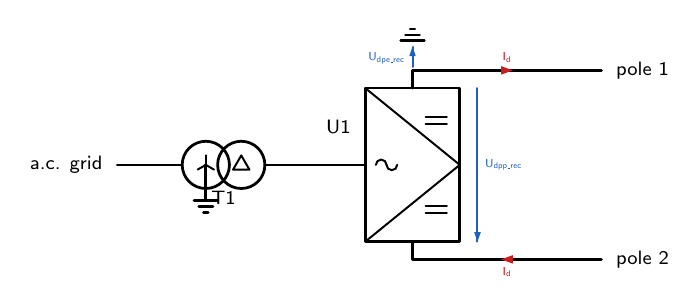
\begin{tikzpicture}[x=1mm, y=1mm, scale=0.6, gw/fig]
  \pic[transform shape, rotate=0, gw/element=T1] (T1) at (-40.0,0.0) {gw/xfmr2-YNd11-e1};
  \node[gw/label, anchor=north] at (T1-tag) {T1};
  \pic[transform shape, rotate=0, gw/signals={udpe_p, udpp, id_p, id_n}, gw/text={label={VSC}}, gw/element=U1] (U1) at (0.0,0.0) {gw/vsc2-sig};
  \node[gw/label, anchor=east] at (U1-tag) {U1};
  \draw[gw/normal] (-52.5,0) -- (-62.5,0);
  \draw[gw/normal] (-27.5,0) -- (-15,0);
  \draw[gw/normal] (25,20) -- (40,20);
  \draw[gw/normal] (25,-20) -- (40,-20);
  \node[gw/label, anchor=east] at (-65,0) {a.c. grid};
  \node[gw/label, anchor=west] at (42.5,20) {pole 1};
  \node[gw/label, anchor=west] at (42.5,-20) {pole 2};
\end{tikzpicture}

\end{verbatim}}
      \begin{itemize}
        \setlength{\itemsep}{0.4em}
        \item \atmono{gw/signals}, \atmono{gw/hide signals}: which signals are drawn.
        \item \atmono{gw/text}: their names; \atmono{gw/sig/<name>}: colour, line style.
        \item Without an override the selection of the YAML file applies.
      \end{itemize}
    \end{column}
    \begin{column}{0.46\textwidth}
      \centering
      \vspace{1.2em}
      {\tikzset{gw/element/U1/.style={
         gw/signals={udpp, id_p},
         gw/text={udpp={U\textsubscript{dc}}},
         gw/sig/udpp/.style={dashed}}}%
       \resizebox{\linewidth}{!}{\slfig{converter-station}}}

      \vspace{0.4em}
      {\color{atGray}\scriptsize The converter station of the diagram slides, with the override on the left.}
    \end{column}
  \end{columns}
\end{frame}


% ---- Transformers -------------------------------------------
\begin{frame}{Transformers\\Variants of one parametric family}
  \noindent{\color{atGray}\small IEC 60617 symbols; the ID selects windings, vector group, neutral treatment and tap changer, the ports stay in place.}
  \vspace{0.8em}

  \centering
  \slfig{transformers}

  \vspace{0.3em}
  \raggedright
  \begin{itemize}
    \setlength{\itemsep}{0.4em}
    \item ID pattern \atmono{xfmr2|3-<vector group>[-e<n>][-oltc]}; \atmono{e1} earths the HV neutral.
    \item Two-, three-winding and autotransformers; illegal combinations are rejected.
  \end{itemize}
\end{frame}


% ---- Switchgear & apparatus ---------------------------------
\begin{frame}{Switchgear \& Apparatus\\IEC 60617}
  \noindent{\color{atGray}\small Circuit breaker, disconnector, earthing switch, surge arrester, voltage and current transducer, cable sealing end and bushing.}
  \vspace{0.6em}

  \centering
  \slfig{switchgear}

  \vspace{0.3em}
  \raggedright
  \begin{itemize}
    \setlength{\itemsep}{0.4em}
    \item Switching devices kept compact beside transformer and converter: breaker and disconnector 10\,mm.
    \item Arrester and voltage transducer optionally earthed (\atmono{-e}); switchgear open or \atmono{-closed}.
  \end{itemize}
\end{frame}


% ---- Converters ---------------------------------------------
\begin{frame}{VSC Converter\\IEC 62747 and signal notation}
  \begin{columns}[T,onlytextwidth]
    \begin{column}{0.50\textwidth}
      \begin{block}{Two layouts}
        Compact square for overview diagrams; tall layout with room for the d.c. notation of the design documents.
      \end{block}
      \vspace{0.3em}
      \begin{itemize}
        \setlength{\itemsep}{0.4em}
        \item Signals selectable one by one: $U_{dpe\_rec}$ pole to earth, $U_{dpp\_rec}$ pole to pole, $I_{d}$ d.c. current.
        \item Voltages blue, currents red; every text is editable per drawing.
        \item The $\sim$ and $=$ marks can stay upright when the symbol is rotated.
      \end{itemize}
    \end{column}
    \begin{column}{0.46\textwidth}
      \centering
      \slfig{converters}
    \end{column}
  \end{columns}
\end{frame}


% ---- Orientation --------------------------------------------
\begin{frame}{Orientation\\Rotation and mirroring}
  \noindent{\color{atGray}\small Every symbol turns in 90° steps and mirrors; texts stay horizontal and readable, ports move with the geometry.}
  \vspace{0.8em}

  \centering
  \slfig{orientation}

  \vspace{0.6em}
  \raggedright
  \begin{itemize}
    \setlength{\itemsep}{0.4em}
    \item Name suffixes \atmono{-r90}, \atmono{-fh} (left--right), \atmono{-fv} (top--bottom), combinable: \atmono{es-fh-r90}.
    \item In a diagram: \atmono{rot: 90} (positive = clockwise), \atmono{flip: h}, \atmono{marks: upright}.
  \end{itemize}
\end{frame}


% ---- SLD: transformer bay -----------------------------------
\begin{frame}{Single-Line Diagram\\Transformer bay}
  \noindent{\color{atGray}\small Busbar to converter from one YAML file, shown in three parts (read left to right): 13 elements, wires and junction dots routed automatically.}
  \vspace{0.6em}

  \centering
  \begin{tabular}{@{}c@{\hspace{2.2em}}c@{\hspace{2.2em}}c@{}}
    \raisebox{-\height}{\slfig{transformer-bay-1}} &
    \raisebox{-\height}{\slfig{transformer-bay-2}} &
    \raisebox{-\height}{\slfig{transformer-bay-3}} \\
  \end{tabular}
\end{frame}


% ---- SLD: converter station ---------------------------------
\begin{frame}[fragile]{Single-Line Diagram\\Converter station}
  \begin{columns}[T,onlytextwidth]
    \begin{column}{0.44\textwidth}
      {\fontsize{6}{7.2}\selectfont
\begin{verbatim}
instances:
  T1: {symbol: xfmr2-YNd11-e1,
       at: [-40, 0]}
  U1: {symbol: vsc2,
       at: [T1.lv+12.5, T1.lv], by: ac,
       signals: [udpe_p, udpp, id_p, id_n]}
nets:
  - [T1.hv, [T1.hv-10, T1.hv]]
  - [T1.lv, U1.ac]
  - [U1.dc1, [U1.dc1+15, U1.dc1]]
  - [U1.dc2, [U1.dc2+15, U1.dc2]]
labels:
  - {at: [U1.dc1+17.5, U1.dc1],
     text: "pole 1", anchor: west}
\end{verbatim}}
      \vspace{0.2em}
      \noindent{\color{atGray}\scriptsize Positions relative to other elements; \atmono{by: ac} places the converter by its a.c. terminal.}
    \end{column}
    \begin{column}{0.54\textwidth}
      \centering
      \vspace{1.2em}
      \slfig{converter-station}
    \end{column}
  \end{columns}
\end{frame}
